\chapter{Background}\label{ch:background}
%************************************************ 

\section{Neural networks as classifiers}

	One of the most popular use cases of \acs{ANN}s is supervised learning; what distinguishes it from unsupervised learning is the existence of labeled examples that guide the learning stage, against the need to infer all information. Supervised learning can be further divided into classification and regression: the former aims to split a set of data into two or more groups, while the latter is more of a function approximation. Since our job will consist in recognizing several types of \acs{EEG} patterns, the discussion will focus on the particular details of classification from here on.

	A neural network, in its most basic form, is made of simple processing units (called \textit{neurons}) distributed among three kinds of layers:

	\begin{itemize}

		\item
		Input layer: with as many neurons as characteristics describing a single sample. Each unit receives the value of its corresponding characteristic as is. Depending on the problem (and not just for this sort of model), it may be useful to preprocess the data so as not to bias the model.

		\item
		Output layer: the number of possible outputs dictates its number of neurons. Only one of them can be active at a time, indicating the answer of the neural network to the classification question.

		\item
		Hidden layers: these are inserted between the previous two. Their quantity ranges from one to hundreds in the most extreme applications, and their interactions yield the predictive ability of the model.

	\end{itemize}

	A typical vanilla feed-forward neural network contains directed connections between its different layers, but not between components of the same layer. Also, the term \textit{feed-forward} implies that there are no cycles in the graph of the network, and so the information moves from the input to the output through the hidden layers. The way in which this information flows is defined by the \textit{weights} of the connections between neurons: although it is frequent to have fully-connected layers, it does not mean that one unit passes the same value to all the other units it points to, or even that it is not null; determining that is precisely the task of the learning algorithm.

\newpage

	To get a better picture of the concept, the following figure illustrates a generic model with one hidden layer:

	\vspace{0.2cm}

	\begin{figure}[bth]

        \myfloatalign
        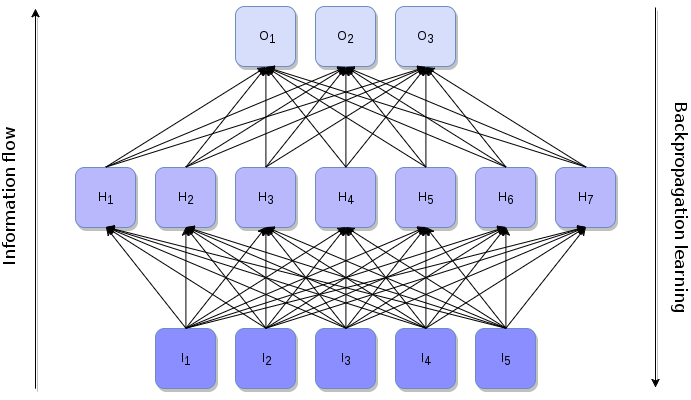
\includegraphics[width=0.95\textwidth]{gfx/NeuralNetwork.png}
        \caption{A neural network with one hidden layer.}

    \end{figure}

    We can see that the hidden layer has its neurons labeled $H_i$. The input layer is represented by the $I_i$ units and the output layer corresponds to the different $O_i$. 

    This image also introduces a new concept: \textit{backpropagation}. Whereas the information is transformed by means of the weights and transmitted forward, the adjustment of those weights needs of a propagation in the opposite direction.